 

  
  
\section{Summary}

The ability to remember and navigate spatial environments is critical for everyday life. A primary mechanism by which the brain represents space is through hippocampal place cells, which indicate when an animal is at a particular location \citep{OKeeDost71}. An important issue is understanding how the hippocampal place-cell network represents specific properties of the environment, such as signifying that a particular position is near a doorway or that another position is near the end of a corridor. The entorhinal cortex (EC), as the main input to the hippocampus, may play a key role in coding these properties because it contains neurons that activate at multiple related positions per environment \cite{FranEtal00,HaftEtal05,DerdEtal09,SolsEtal08,BjerEtal14}.  We examined the diversity of spatial coding across the human medial temporal lobe by recording neuronal activity during virtual navigation of an environment containing four similar paths. Neurosurgical patients performed this task as we recorded from implanted microelectrodes, allowing us to compare the human neuronal representation of space with that of animals. EC neurons activated in a repeating manner across the environment, with individual cells spiking at the same relative location across multiple paths. This finding indicates that EC cells represent non-specific information about location relative to an environment's geometry, unlike hippocampal place cells, which activate at particular random locations. Given that spatial navigation is considered to be a model of how the brain supports non-spatial episodic memory \cite{EichLipt08,BirdBurg08,Hass12,BuzsMose13}, these findings suggest that EC neuronal activity is used by the hippocampus to represent the properties of different memory episodes \cite{FranEtal00,BuckEtal04}.




\section{Results}
We recorded 1,329 single neurons in various brain regions from 13 neurosurgical patients performing a virtual-navigation task.  Patients were instructed to learn an environment's layout and navigate between six destination ``stores''  as rapidly and accurately as possible. This environment was a square track (see Figure~\ref{fig:behaviorCurrBio}A), which limited the patients' navigation path to particular regions of the environment. Navigation errors decreased across trials of the task (Figure~\ref{fig:behaviorCurrBio}B), indicating that patients successfully learned the environment's layout.
  

\begin{figure} \centering 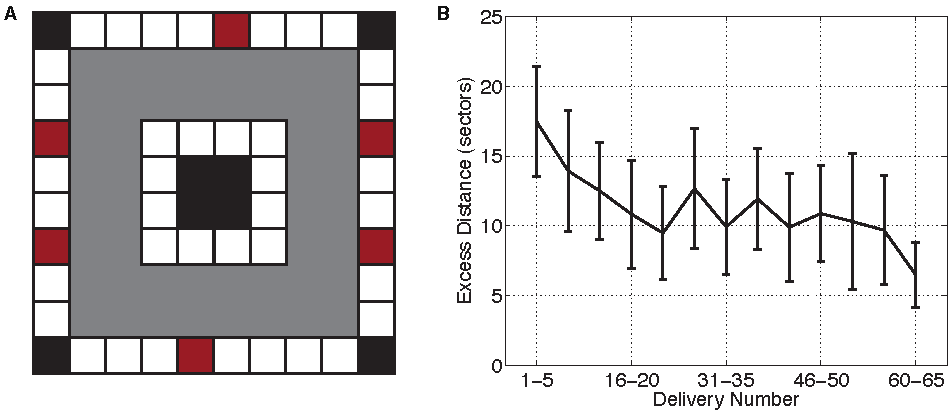
\includegraphics[width=.9\textwidth]{./tex/linearGrids/figs/Figure1} \caption[Behavioral task and performance]{\textbf{Behavioral task and performance.} \textbf{(A)} An overhead schematic of the layout of the virtual environment. Red squares represent locations of the destination stores and white square are non-store buildings. Gray shading indicates regions of the environment where the patient could travel. \textbf{(B)} Subject average task performance as a function of delivery trial number. Performance is measured as the excess number of sectors traveled when searching for a destination store, compared to an ideal path. Error bars are 95\% confidence intervals. See also Figure S1.} \label{fig:behaviorCurrBio}
\end{figure}


Our main objective was to characterize how the spiking of individual neurons varied to represent  the patient's virtual spatial location. For each cell, we computed firing rate maps corresponding to the cell's mean rate of spiking as a function of the current  virtual location. A previous analysis of this dataset \cite{JacoEtal10} revealed  many \emph{path cells}, which coded for whether the participant was traveling clockwise or counterclockwise around the track. Thus, we computed firing rate maps separately for movements in clockwise and counterclockwise directions. We  calculated these maps  in a smoothed manner, as well as in a discretized manner that binned the patients' location into one of 25 sectors on each side of the track.

Next, we identified cells that significantly varied their firing rate according to the patient's virtual location. We used a one-way ANOVA as a screening procedure to identify individual neurons whose firing rates varied in response to the current sector of the environment. According to this measure, 313  cells (23.5\%) were responsive to the location, a percentage that is in line with previous single-cell studies of human virtual navigation \cite{EkstEtal03,JacoEtal10,JacoEtal13}. Our subsequent analyses focused on more precisely characterizing the activity of these cells.


A distinctive feature of some location-responsive cells in rodents is that they activate at multiple  spatial locations that are related to each other, such as positions just before or after a curve \cite{FranEtal00}, locations at particular distances from borders \cite{SolsEtal08,DerdEtal09,BjerEtal14}, or spots associated with particular landmarks \cite{HargEtal05,TsaoEtal13}.  We sought to identify analogous  types of representations in humans by searching for cells that exhibited significant \emph{path equivalence} across distinct sections of the virtual environment \cite{FranEtal00}.  We computed the path-equivalence coefficient for each cell, which is a measure of the similarity of the cell's firing activity across two or more corridors (see \emph{Experimental Procedures}).  A cell that exhibited significant path equivalence is one that activated at the same relative position on multiple sides, such as a cell that spiked when a person was passing through the midpoint of any of the four paths.  Of the 313 location-responsive cells, 30 (9.6\%) exhibited significant path-equivalent firing patterns ($p<0.001$).


\begin{figure}[t]
\centering
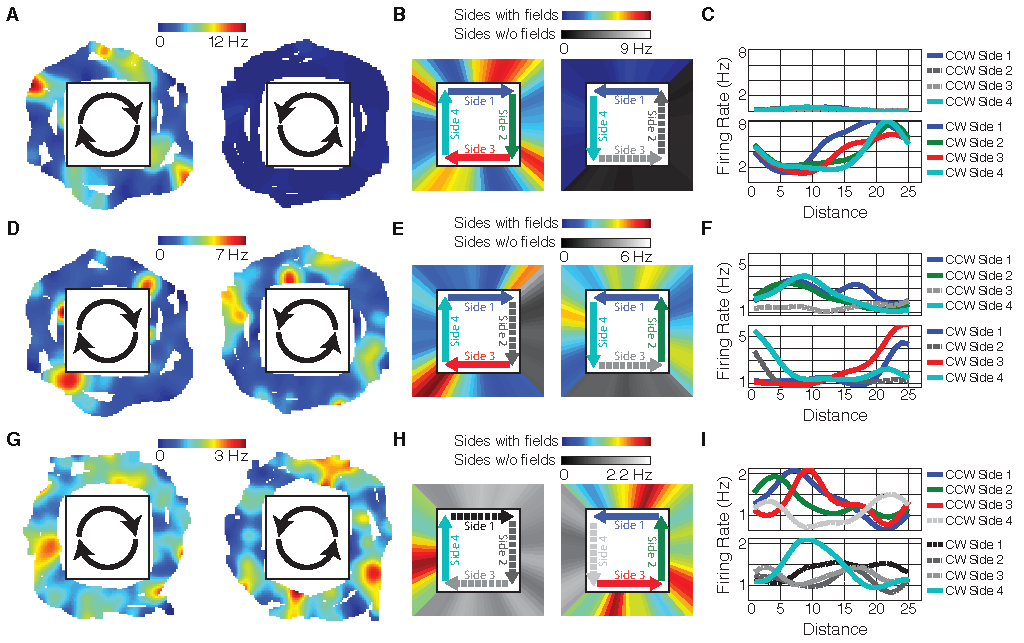
\includegraphics[width=.99\textwidth]{./tex/linearGrids/figs/Figure2}
\caption[Path equivalent cell firing rate maps]{\textbf{Path equivalent cell firing rate maps.} \textbf{Top Row:} Activity of a cell in patient 2's entorhinal cortex. \textbf{(A)} Two dimensional firing rate map for epochs of clockwise (left) and counterclockwise (right) movement. \textbf{(B)} Linearized firing rate maps (smoothed with a 12-pt window) for epochs of clockwise (left) and counterclockwise (right) movement. Sides with regions of significantly elevated firing are shown in color, and sides without significant activations are in grayscale. \textbf{(C)} Firing rate as a function of distance from the beginning of the side, plotted separately for each side of the environment and for clockwise (bottom) and counterclockwise (top) directions. \textbf{Middle Row:} Activity of a cell in patient 2's  entorhinal cortex. \textbf{Bottom Row:} Activity of a cell in patient 5's cingulate cortex. See also Figure S2.}
\label{fig:firingExamples}
\end{figure}

Three example path equivalent cells are shown in Figure~\ref{fig:firingExamples}. Figure~\ref{fig:firingExamples}A--C highlights one cell in the EC that activated consistently as the patient approached the end of each corridor during clockwise movement. Figure~\ref{fig:firingExamples}D--F shows a different cell in the EC that activated at similar locations across multiple corridors, with the locations of activations shifting between clockwise and counterclockwise movements. Figure~\ref{fig:firingExamples}G--I illustrates a cell from cingulate cortex that activated near the beginning of multiple corridors during counterclockwise movement. Additional example cells are shown in Figure~\ref{fig:otherExamples}.

We found significant levels of path-equivalent cells in only two regions: the entorhinal cortex and the cingulate cortex (Figure~\ref{fig:population}A).  The magnitude of individual cells' path-equivalent firing was greater in EC compared to cingulate cortex, as indicated by the fact that the mean path-equivalence coefficient for EC path-equivalent cells (0.92) was greater than for path-equivalent cells in cingulate cortex (0.49; $p<.05$, rank-sum test). We specifically compared the level of path-equivalent activity between the hippocampus and its main input, the entorhinal cortex, and found that the entorhinal cortex contained more path-equivalent cells than the hippocampus ($p<0.05$, post-hoc $\chi^2$ test). This difference in the prevalence of path-equivalent cells cannot be attributed to a difference in the stability of the spatial coding between EC and hippocampus, as these two regions did not differ in the percentage of location sensitive cells that were stable over time (45\% EC vs 53\% hippocampus, n.s.).  Prior research suggested functional differences across regions within the entorhinal cortex \cite{HaftEtal05,HargEtal05,BrunEtal08a}.  However, we did not find any difference in the proportion of path-equivalent cells between neurons located in the posterior vs.\ anterior EC, lateral vs.\ medial, or superior vs.\ inferior positions ($\chi^2$ tests, all $p$'s$ > 0.1$).

\begin{figure}[t]
\centering 
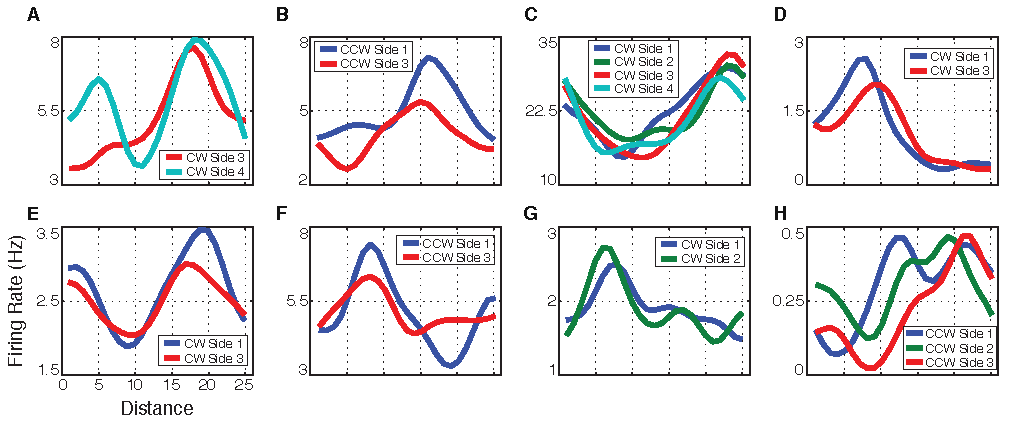
\includegraphics[width=.99\textwidth]{./tex/linearGrids/figs/Figure3}
\caption[Examples of path equivalent cells]{\textbf{Examples of path equivalent cells.} \textbf{(A)} A cell from patient 1's cingulate cortex during clockwise movement. \textbf{(B)} A cell from patient 2's entorhinal cortex during counterclockwise movement. \textbf{(C)} A cell from patient 2s entorhinal cortex during clockwise movement. \textbf{(D)} A cell from patient 5's entorhinal cortex during clockwise movement. \textbf{(E)} A cell from patient 10's parahippocampal gyrus during clockwise movement. \textbf{(F)} A cell from patient 12's entorhinal cortex during counterclockwise movement. \textbf{(G)} A cell from patient 13's hippocampus during clockwise movement. \textbf{(H)} A cell from patient 13's hippocampus during counterclockwise movement. See figure S3 for additional examples.} \label{fig:otherExamples}
\end{figure}


The path-equivalence measure we employed is sensitive to the overall shape of a cell's firing pattern.  Thus, this measure could be influenced by cells with diffuse firing patterns \cite{QuirEtal92} rather than the spatially precise activations  of conventional place or grid cells.  To verify that the pattern of path-equivalent cells we observed was driven by the locations of peak spatial activations, we directly tested whether the relative locations of peak firing  (place fields) were maintained across the sides of the environment. We identified each cell's place fields and then computed, for each cell, the percent of pairs of corridors of the environment where the relative locations of the place fields overlapped by at least 50\% (Figure~\ref{fig:population}B).  This analysis supports  the finding that the EC plays a particular role in path equivalence because cells in EC had the greatest percent of corridors where place fields were located at the same relative location. Across all cells with place fields on two or more corridors in the EC, 40\% of the possible corridor pairs had fields in overlapping locations. This is significantly more than the  22\% of corridor pairs for cells in cingulate cortex ($p<.05$, ranksum test). If we restrict this analysis to only the previously identified path-equivalent cells, the difference is more pronounced (87\% compared to 47\%).

One possibility is that individual neurons do not represent particular locations but rather that these  signals actually encode distance traveled.  We compared the location- or distance-encoding hypotheses  by comparing the firing patterns of neurons that exhibited place fields during both clockwise and counterclockwise directions. For the 25 path-equivalent cells that met this criterion, we computed the correlation between the mean clockwise and counterclockwise firing patterns. We distinguished distance and location-based firing by computing this correlation two ways: with the firing rate vectors aligned by absolute location, and with the vectors ordered by distance along the direction of movement. A positive correlation in the first case indicates location coding, whereas a positive correlation in the second indicates distance coding. Of the path-equivalent cells analyzed, 11 (44\%) showed significant correlations. Of these 11, 8 showed distance coding  (e.g., Fig.~\ref{fig:firingExamples}I), 1 showed location coding, and 2 were ambiguous. This result supports the hypothesis that some path-equivalent cells  play a role in representing relative distance  ($p<.05$, $\chi^2$ test).




\begin{figure}[t]
\centering
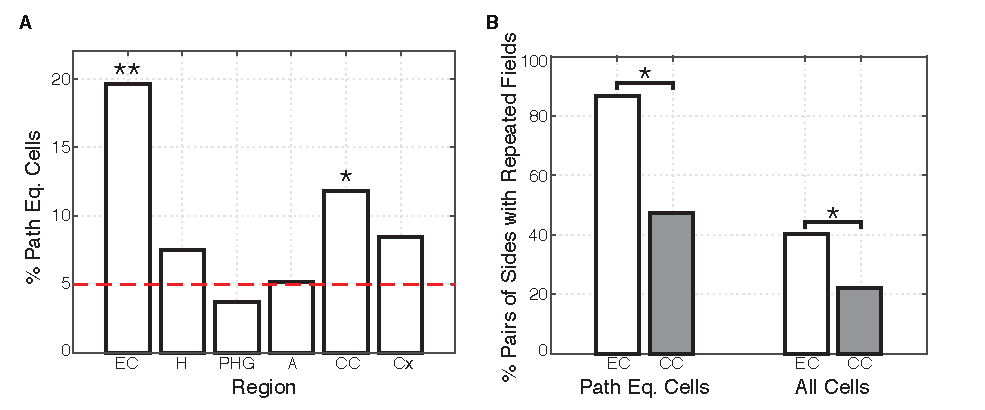
\includegraphics[width=.99\textwidth]{./tex/linearGrids/figs/Figure4}
\caption[Population measurements]{\textbf{Population measurements.}  \textbf{(A)} Regional distribution of \emph{path-equivalent cells}, which are location-responsive cells that have correlated responses across multiple corridors in the environment. EC: entorhinal cortex; H: hippocampus; PHG: parahippocampal gyrus; A: amygdala; CC: cingulate cortex; Cx: frontal/lateral-temporal cortex. \textbf{(B)} The percent of corridor pairs with place fields at the same relative locations.  This measure is computed by identifying each cell with place fields on at least two corridors and measuring, across all pairs of corridors, how often place fields occur at the same relative location.  $**$ denotes $p<.0001$, $*$ denotes $p<.05$. See also Figure S4 and Table S1.}
\label{fig:population}
\end{figure}


\section{Discussion}

We examined human single-neuron recordings during virtual navigation and found a set of location-responsive cells that exhibited repeated firing patterns across multiple related areas of an environment. The key feature of these path-equivalent cells is that they consistently activated at the same relative position across separate corridors.  This  is the first evidence in humans that individual cells  generalize features across multiple  settings.  By activating at multiple locations, these cells behave very differently from place cells, which activate at only one location per environment. Because path-equivalent cells are input to the hippocampus, it indicates that a critical function of the human hippocampus is to build distinctive neuronal representations from non-specific entorhinal input. An additional contribution of our work is showing that  humans exhibit clear spatially modulated neuronal firing in \emph{virtual} navigation, supporting the view that virtual and physical navigation are supported by some similar mechanisms, as previously  demonstrated in rodents in various brain structures \cite{AghaEtal14,HarvEtal09,RavaEtal13}.


Our demonstration of EC path-equivalent cells complements previous studies describing rodent neurons with repeating spatial firing patterns. One example is a study by \citet{DerdEtal09}, which measured the activity of entorhinal grid cells as rodents navigated a constrained track. During movement in one direction of a hairpin maze, grid cells activated to represent equally spaced groups of locations that were consistently positioned across multiple corridors. As that paper demonstrates, grid cells generally reset their grids at  entrances to individual corridors,  giving rise to the appearance of a repeating  pattern across different sections of the environment. Some of the cells in our study appear to exhibit a similar pattern, in which they reset their representation upon entering each corridor. This supports the view that the neural representation of space can be segmented by  entrances to different compartments  \cite{FranEtal00,SpieEtal13}.  

Our findings are also related to data from \citet{FranEtal00}, who reported path-equivalent cells in rodent EC.  The path-equivalent cells described in that study activated at analogous locations both within and across environments.  Although several aspects of our findings are similar to the cells from that study, one critical difference is that when path-equivalent cells activate, the rat always has the same compass-like absolute heading.  In contrast, for the path equivalent cells that we report, each activation corresponds to a circular heading and location within the environment.  In a previous study from this dataset, we reported \emph{path cells} that encoded direction in a circular manner such that they activated during either clockwise or counterclockwise movement \citep{JacoEtal10}.  Thus, one possibility is that the entorhinal representation of direction in humans can be transformed according to an environment's layout so that it may depart from a fixed compass-like orientation scheme. Although human EC path-equivalent share features with grid cells, it is premature to conclude that the data reported here are from grid cells.  As we demonstrate in \emph{Figure S2}, owing to the four-way symmetry of our square environment, our data are not consistent with a grid cell that encoded the patient's position using a triangular coordinate system in two-dimensional space.  We could not test whether the cells in our dataset exhibit grids aligned  individual corridors \cite{DerdEtal09} because the length of each corridor was too short to observe a possible grid repetition.
 
As studies of rodent spatial navigation characterize the functional relationship between different brain regions, theories of hippocampal function are converging on the idea that rodent spatial navigation is a model for studying other aspects of cognition, including episodic memory \citep{EichEtal99,Buzs05,BuzsMose13,MoseMose13}. These theories share the idea that the representation of specific episodic memories can be considered analogous to the representation of locations by place cells. The role of the EC in this system may be to represent non-specific features of the behavioral setting \citep{HaftEtal05,SolsEtal08,SargEtal06,JacoEtal13,JacoEtal10} for encoding into specific memories (or locations) by the hippocampus \cite{NormORei03}. During navigation, EC neurons may  represent the attributes of a setting, with each cell activating at related   locations, as in our findings and in some earlier animal work  \cite{FranEtal00}.  To our knowledge, our findings are the first demonstration of this type of featural neuronal coding in the human EC (cf.\ Mormann et al., 2008 \cite{MormEtal08}). By demonstrating a key difference between hippocampal and entorhinal representations during navigation, our results support theoretical models regarding the diversity of information processing throughout the medial temporal lobe \cite{NormORei03,KnieEtal06,SolsEtal06}. 
 



\section{Experimental Procedures}

\paragraph{Participants and Task Design.} The task design and methods for data acquisition are described in a previous study that examined this same dataset \citep{JacoEtal10}. All data analyses and results reported here are novel, although the prior study \citep{JacoEtal10} did qualitatively describe the activity of one cell we examined here. Thirteen patients undergoing surgical treatment for medication-resistant epilepsy participated in the study.  All surgeries were performed by I.F. and the research protocol was approved by the University of California, Los Angeles Institutional Review Board.  Patients played a 3D virtual navigation game on a laptop computer in their hospital room \citep{EkstEtal03,JacoEtal10,JacoKaha10,JacoEtal13}. The virtual environment consisted of six destination stores surrounding the perimeter of a square track, with the center of the environment obstructed by buildings (Figure~\ref{fig:behaviorCurrBio}A). On each delivery trial the patient transported a passenger to their requested store destination as accurately as possible.  After arrival at the destination, on-screen text displayed the name of the next randomly selected destination store.

\paragraph{Electrophysiology.}  We recorded spiking activity at 28--32~kHz using 40-$\mu$m platinum-–iridium microwire electrodes \citep{FrieEtal99} connected to a Neuralynx recording system. Nine microwires extended from the tip of each clinical depth electrode. Action potentials were manually isolated using spike shape, clustering of wavelet coefficients, and interspike intervals \citep{QuirEtal04}.  We localized the locations of individual electrodes by co-registering post-operative CT scans with pre-implant MRI images and standardizing to a normalized brain \cite{TalaTour88}.

\paragraph{Data Preprocessing.} We binned the firing rate of each cell into 100-ms epochs. We labeled each epoch with the patient's location and direction of travel (either clockwise or counterclockwise around the square path). With the exception of the firing-rate maps presented in Figure~\ref{fig:firingExamples}A,D,G, all data analyses were conducted after linearizing patients' location into 100 discrete sectors (25 per side) along the square path.

\paragraph{Data Analysis.}
For each cell, we computed a one-way ANOVA as a screening procedure to identify cells whose firing rate varied significantly according to environment sector, assessing significance with a shuffling procedure \cite{EkstEtal03}. 
To determine whether a cell displayed a similar firing patterns across multiple sides of the square track, we used a modified version of the path equivalence coefficient from Frank et al.\ \citep{FranEtal00}. The path equivalence coefficient is a measure of the degree to which a cell fires in similar relative locations on multiple trajectories. Only sides of the track that contained at least one region of three or greater contiguous sectors of elevated firing were included.  We define the path-equivalence coefficient as the median correlation between the firing rates of all pairs of included sides minus the median correlation between the firing rates of all pairs of included sides and shuffled sides:

\(median(corr(side_{i},side_{j})) ~~ - ~~ median(corr(side_{i},shuf_{j}))\)

where $side$ is the firing rate of the corresponding 25 sectors, $shuf$ is the firing rate of the corresponding 25 sectors shuffled as described below, and $i$ and $j$ range from 1 to the number of included sides. To determine the firing rate values of a  shuffled side, the corresponding  firing rate values for the first half of that side were reversed and then the values of the two halves were swapped (e.g., a path of locations   ``A..BC..D''  become ``C..DA..B''). Statistical significance was determined using a permutation procedure (see \emph{Supplemental Experimental Procedures}).

\section{Supplemental Data}

\begin{figure}[bh]
\begin{center}

\includegraphics[width=.6\textwidth]{./tex/linearGrids/figs/supp_occupancy}
\caption[Average occupancy map]{Average occupancy map across all sessions. Brighter shading represents a greater amount of time spent in the region.}
\end{center}
\end{figure}

\begin{figure}[bh]
\begin{center}
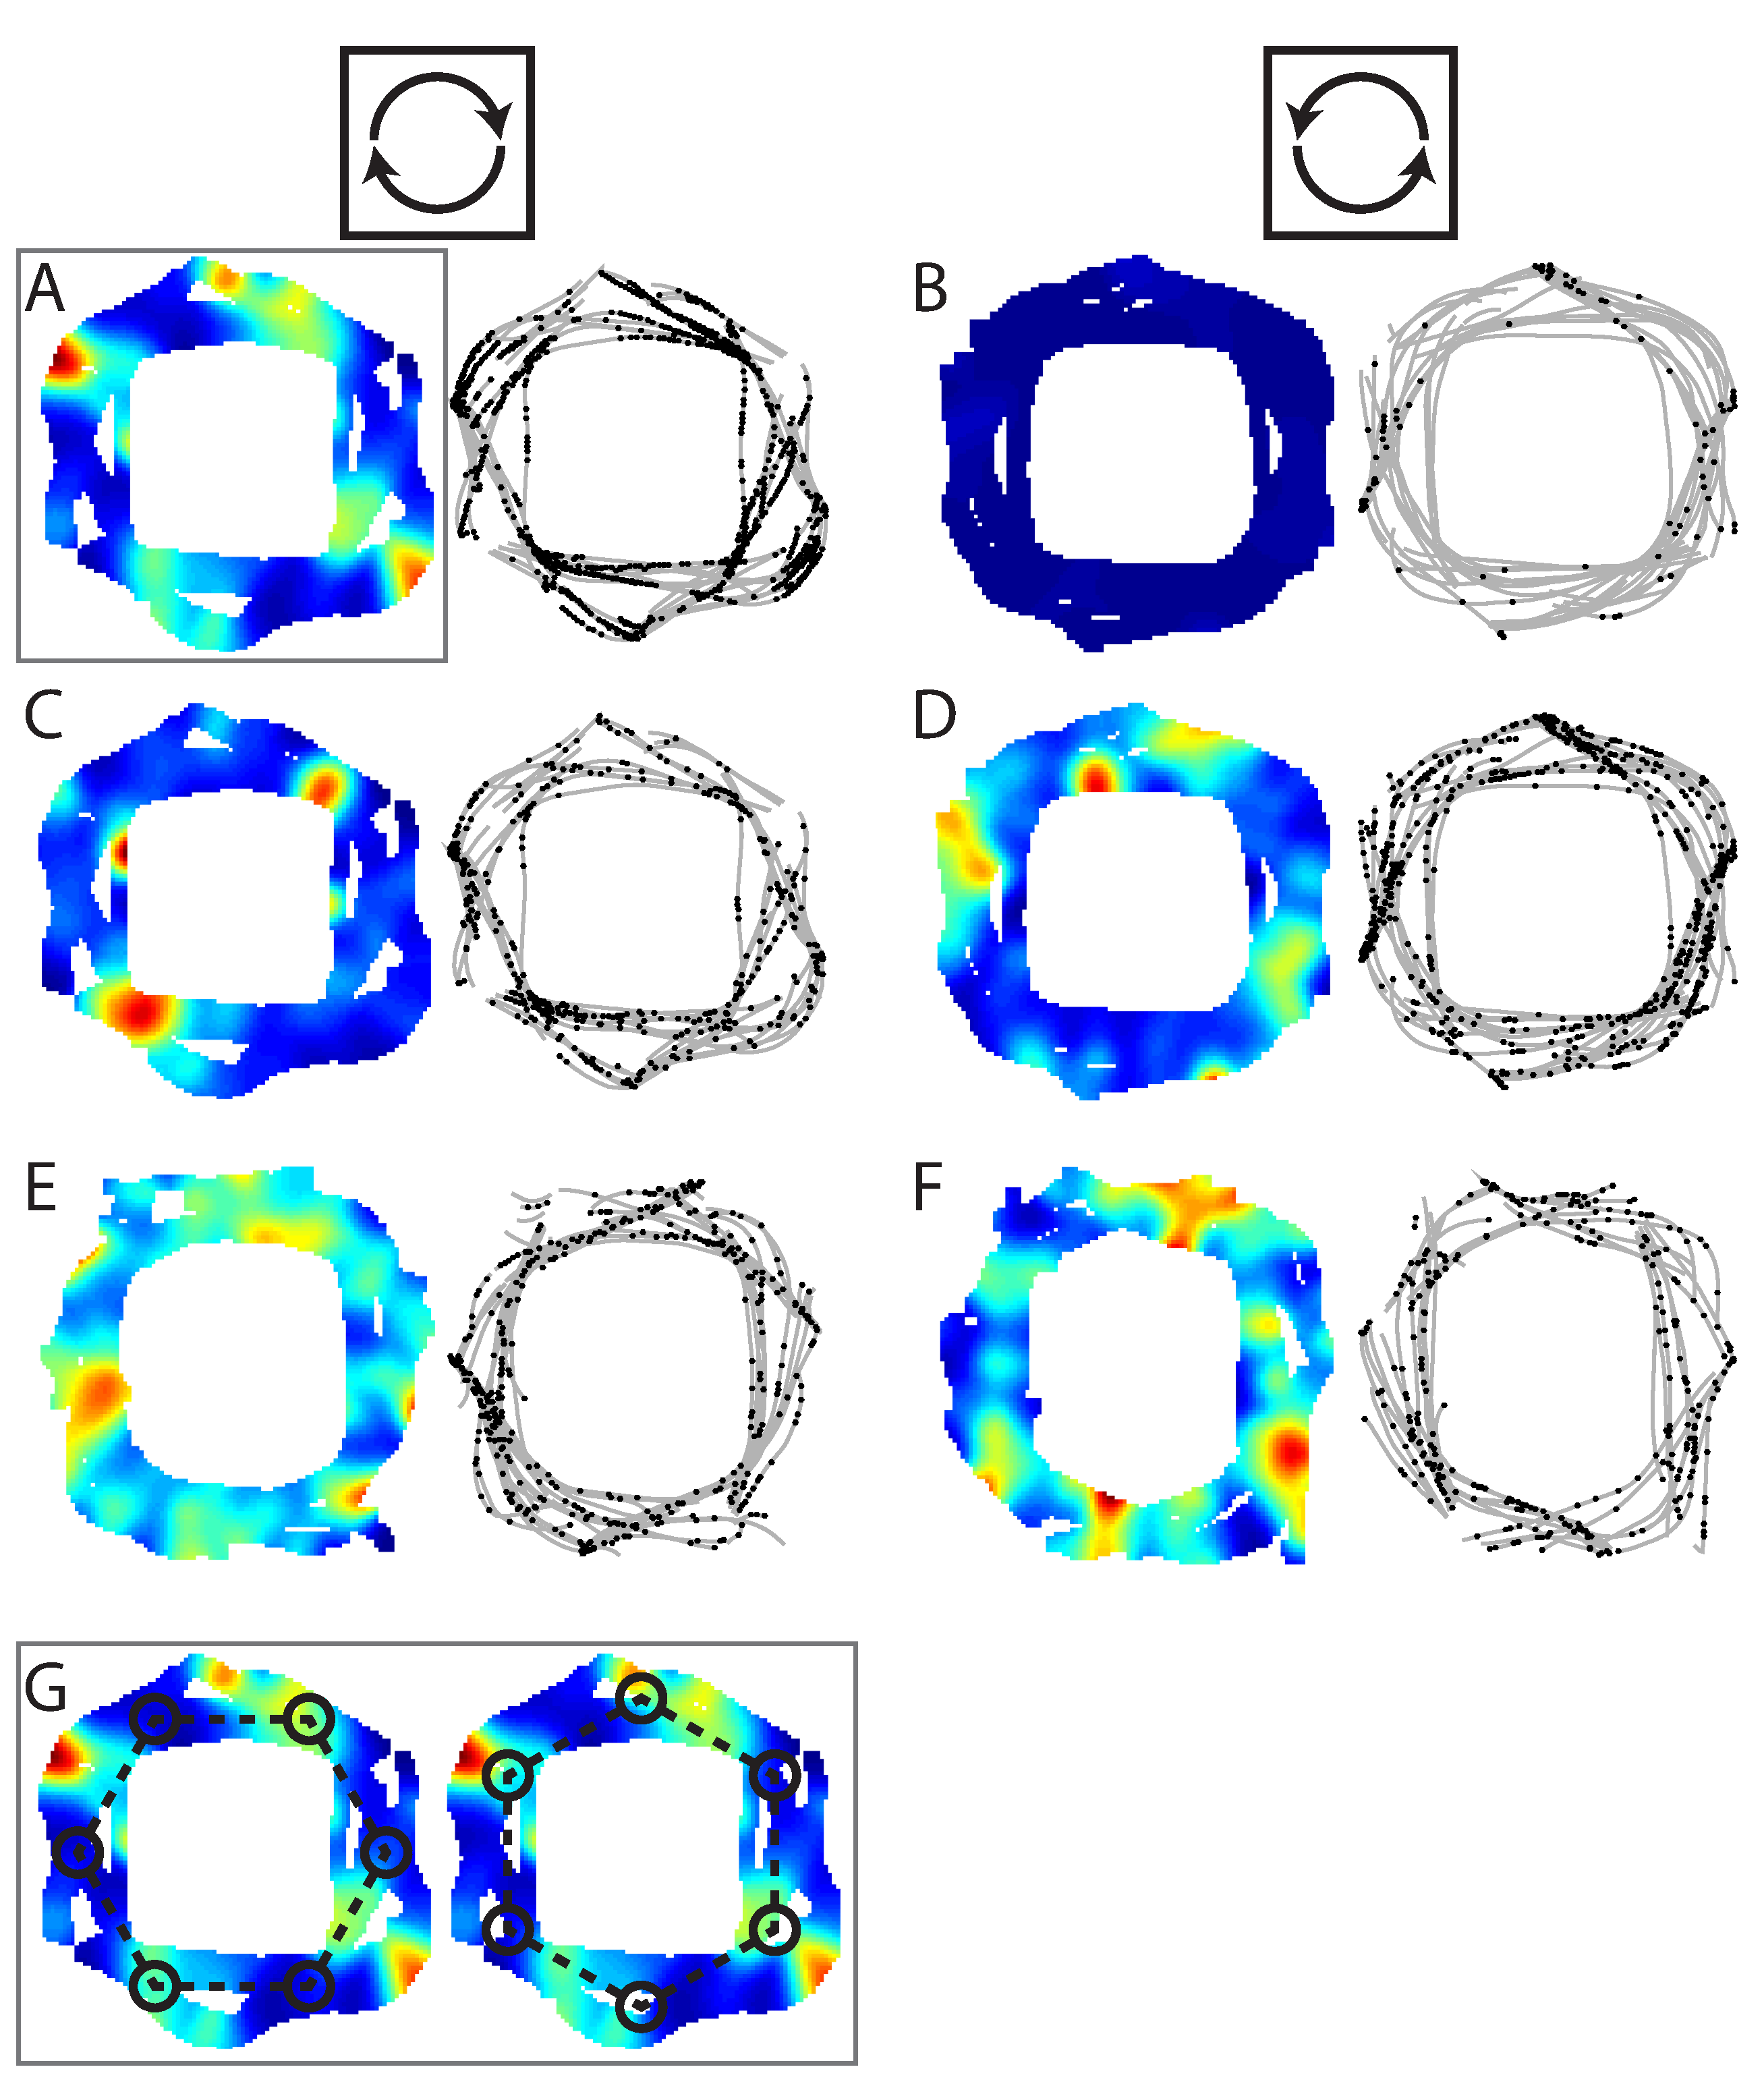
\includegraphics[width=.95\textwidth]{./tex/linearGrids/figs/supp_with_dots.pdf}
\caption[Firing rate maps and associated spiking activity]{\textbf{Firing rate maps and associated spiking activity. A-F. } The rate maps from Figure 2 of the main text are replotted (left) along with the paths taken by the subject and locations where the cell fired, indicated by the gray lines and black dots, respectively (right). \emph{A,C,E:} Clockwise activity for the cells shown in Figure 1. \emph{B,D,F:} Counterclockwise activity for the cells shown in Figure 1. \textbf{G. } Firing rate map with an overlaid hexagon for a cell from patient 2's entorhinal cortex (as shown in panel A). The hexagon vertices do not closely fit the locations of the firing peaks, which suggests that our findings are not driven by a conventional grid cell that activates as if in an open arena. \emph{Left:} Unrotated hexagon. \emph{Right:} Hexagon rotated 30 degrees.}
\end{center}
\end{figure}

\clearpage
\begin{figure}[bh]
\centering
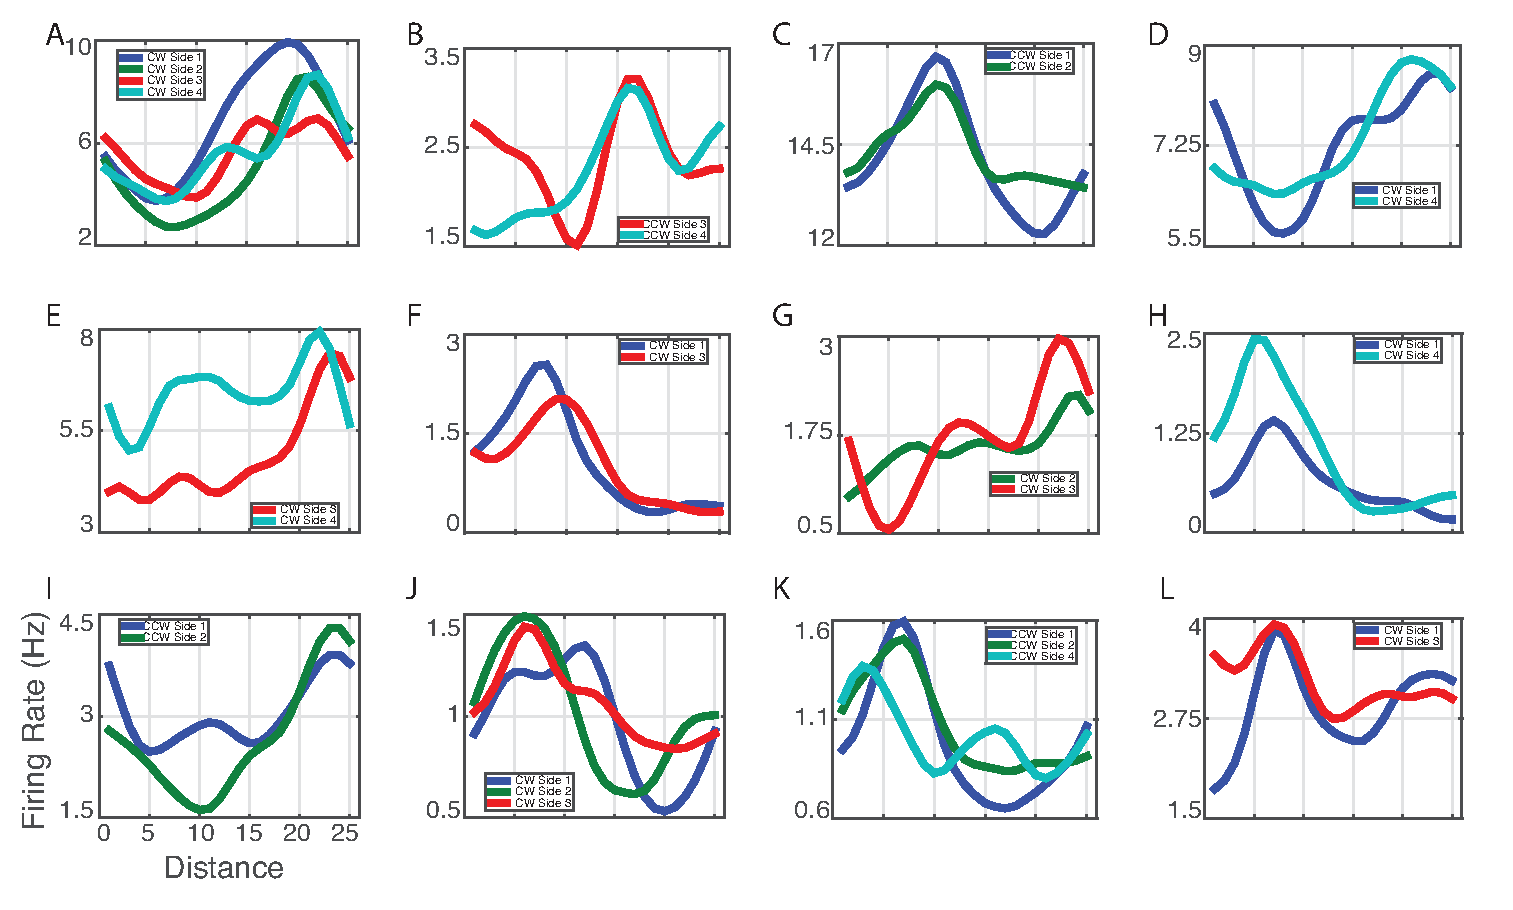
\includegraphics[width=1\textwidth]{./tex/linearGrids/figs/supp_extra_cells_large}
\caption[Additional examples of path equivalent (PE) cells]{\textbf{Additional examples of path equivalent (PE) cells.} \textbf{(A)} A PE cell from patient 2. \textbf{(B)} A PE cell from patient 3. \textbf{(C)} A PE cell from patient 3. \textbf{(D)} A PE cell from patient 4. \textbf{(E)} A PE cell from patient 4. \textbf{(F)} A PE cell from patient 5. \textbf{(G)} A PE cell from patient 6. \textbf{(H)} A PE cell from patient 6. \textbf{(I)}  A PE cell from patient 9. \textbf{(J--K)} One PE cell from patient 10 during two different directions of movement. \textbf{(L)}  A PE cell from patient 11.}
\end{figure}

	
\clearpage
\begin{figure}
\begin{center}
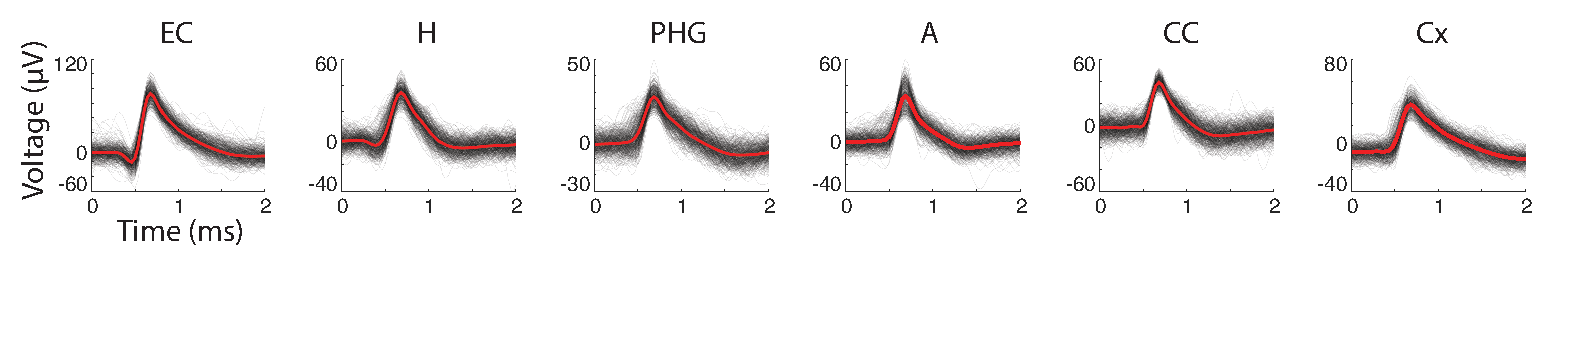
\includegraphics[width=.99\textwidth]{./tex/linearGrids/figs/waveforms}
\scriptsize	
 \begin{tabular}{|c|C{.5cm}|C{1cm}|C{.7cm}|C{.65cm}|C{1cm}|C{.8cm}|C{.8cm}|C{.8cm}|C{.8cm}|C{.8cm}|}
\hline
Region &Mean Firing Rate (Hz) &Firing Rate 5\%-95\% Range (Hz) &Mean Spike Amplitude ($\mu{}V$) &Background noise  ($\mu{}$V) &Mean False Positive (FP) Rate &FP below 10\% &FP below 20\% &Mean False Negative (FN) rate &FN below 10\% &FN below 20\%\\\hline
Entorhinal Cortex &4.0 &0.1-11.9 &44.8 &6.8 &3.7\% &91.1\% &95.6\% &4.2\% &88.6\% &94.9\%\\
Hippocampus &2.5 &0.1-10.3 &42.8 &6.7 &3.5\% &87.0\% &96.8\% &3.7\% &87.7\% &95.4\%\\
Parahippocampal Gyrus &2.0 &0.1-7.6 &36.8 &6.1 &2.0\% &95.7\% &97.9\% &2.6\% &94.7\% &95.7\%\\
Amygdala &2.7 &0.2-9.7 &51.9 &6.7 &7.6\% &77.8\% &88.3\% &7.5\% &77.1\% &88.3\%\\
Cingulate Cortex &4.1 &0.2-11.8 &45.0 &8.0 &6.7\% &79.1\% &89.8\% &7.4\% &76.7\% &86.4\%\\
Frontal/Temporal Cortex &3.2 &0.2-11.2 &42.3 &6.9 &5.0\% &80.3\% &92.2\% &5.1\% &80.3\% &91.9\%\\
\hline
\end{tabular}
\caption[Spike cluster characteristics]{Spike cluster characteristics. \textbf{Top:} Example spike waveforms from each brain region. Red line indicates the mean \textbf{Bottom:} Spike cluster isolation metrics. False-positive rate indicates the estimated percentage of spikes that were inappropriately designated as belonging to a given neuron.  False-negative rate indicates the percentage of spikes that were caused by a given neuron but were inappropriately labeled as belonging to neighboring neurons or noise. We compared the spike waveforms of path-equivalent cells with those of other neurons and did not find any differences in their mean amplitude (41~$\mu V$ for path-equivalent cells vs.\ 45~$\mu V$ for other cells; $p>0.35$, ranksum test) or in our false-positive or false-negative rates in  distinguishing their waveforms from neighboring cells ($p$'s$>0.1$, ranksum tests).}
\end{center}
\end{figure}	
	
\clearpage
\begin{table}
	\begin{center}
	\small
\begin{tabular}{c|cccccc}
Subject \# & EC & H & PHG & A & CC & Cx\\\hline
1 &0 of 0 (0) &0 of 5 (12) &0 of 0 (0) &0 of 3 (20) &1 of 5 (18) &0 of 5 (28)\\
2 &5 of 18 (38) &0 of 6 (27) &0 of 0 (4) &0 of 0 (0) &0 of 9 (40) &0 of 10 (52)\\
3 &0 of 3 (12) &0 of 0 (3) &0 of 0 (0) &0 of 16 (74) &0 of 8 (14) &2 of 10 (47)\\
4 &1 of 6 (32) &1 of 11 (39) &0 of 0 (0) &1 of 5 (39) &2 of 13 (35) &0 of 0 (21)\\
5 &2 of 10 (34) &0 of 7 (45) &0 of 0 (0) &0 of 0 (0) &2 of 7 (38) &0 of 8 (51)\\
6 &1 of 9 (24) &0 of 0 (0) &0 of 0 (0) &1 of 2 (13) &1 of 5 (37) &1 of 10 (32)\\
7 &0 of 0 (0) &0 of 5 (24) &0 of 3 (5) &0 of 7 (23) &0 of 2 (5) &0 of 5 (17)\\
8 &0 of 0 (0) &0 of 6 (39) &0 of 5 (27) &0 of 0 (1) &0 of 0 (0) &0 of 0 (7)\\
9 &0 of 0 (0) &0 of 2 (8) &0 of 0 (0) &0 of 1 (2) &0 of 0 (0) &1 of 3 (9)\\
10 &0 of 0 (0) &1 of 5 (15) &1 of 9 (24) &1 of 9 (28) &0 of 0 (0) &0 of 0 (6)\\
11 &0 of 0 (0) &0 of 6 (26) &0 of 3 (4) &0 of 4 (12) &0 of 2 (19) &1 of 3 (37)\\
12 &1 of 2 (8) &0 of 1 (12) &0 of 3 (22) &0 of 8 (40) &0 of 0 (0) &0 of 0 (0)\\
13 &0 of 3 (10) &3 of 13 (35) &0 of 4 (8) &0 of 3 (14) &0 of 0 (0) &0 of 5 (13)\\
\hline Total &10 of 51 (158) &5 of 67 (285) &1 of 27 (94) &3 of 58 (266) &6 of 51 (206) &5 of 59 (320)\\
\end{tabular}
\caption[Summary of path equivalent cells]{Summary of path equivalent cells by patient and brain region. Counts indicate the number of path equivalent cells out of the total number of location-responsive cells. Numbers in parentheses indicate the total number of cells recorded, regardless of whether a cell was location-responsive. EC: entorhinal cortex; H: hippocampus; PHG: parahippocampal gyrus; A: amygdala; CC: cingulate cortex; Cx: frontal/lateral-temporal  cortex.}
\end{center}
\end{table}


\section{Supplemental Experimental Procedures}

\paragraph{Participants.} The task design and methods for data acquisition were described in a previous study that examined this same dataset \citep{JacoEtal10}. In brief, thirteen patients undergoing surgical treatment for medication-resistant epilepsy participated in the study.  All surgeries were performed by I.F. and the research protocol was approved by the University of California, Los Angeles Institutional Review Board.  Our dataset is comprised of 35 individual testing sessions (30--50 minutes each), with each participant contributing between one and four sessions.  All data analyses and results reported here are novel, although the prior study \citep{JacoEtal10} did qualitatively describe the activity of one cell we examined here.

\paragraph{Behavioral Task.} Patients played a virtual navigation game  \citep{EkstEtal03,JacoEtal10,JacoEtal13} on a laptop computer in their hospital room. The virtual environment consisted of six destination stores surrounding the perimeter of a square track, with the center of the environment obstructed by buildings. Patients traveled either clockwise or counterclockwise around the track. Two stores each were located on the east and west walls (sides 2 and 4), and one store each was on the north and south walls (sides 1 and 3). The stores were all visually distinct. The patients navigated the environment using a game controller. On each delivery trial the patient transported a passenger to their requested store destination as accurately as possible.  After arrival at the destination, on-screen text displayed the name of the next randomly selected destination store.

\paragraph{Electrophysiology.}  We recorded spiking activity at 28--32~kHz using 40-$\mu$m platinum-–iridium microwire electrodes \citep{FrieEtal99} connected to a Neuralynx recording system. Nine microwires extended from the tip of each clinical depth electrode. The first eight wires were insulated except for their tip and were used to record action potentials. The ninth microwire had its insulation stripped for $\sim$1~cm and served as the voltage reference for the other  wires. Action potentials were manually isolated using spike shape, clustering of wavelet coefficients, and interspike intervals \citep{QuirEtal04}.  We localized the locations of individual electrodes by co-registering post-operative CT scans with pre-implant MRI images and standardizing to a normalized brain \cite{TalaTour88}.  Assessing  entorhinal subregions is an  area of ongoing research \cite{KhanEtal14}. The approach we used to localize within the EC was by performing median splits across extent of our EC electrodes in the lateral/medial, anterior/posterior, and ventral/dorsal axes. % localize individual electrodes  For each dimension, we found the minimum and maximum coordinate across all of our EC electrodes, and we classified each electrode based on half of the total range.


\paragraph{Data Preprocessing.} We binned the firing rate of each cell into 100-ms epochs. We labeled each epoch with the patient's location and direction of travel (either clockwise or counterclockwise around the square path). Following previous work on this dataset \cite{JacoEtal07,JacoEtal10}, epochs without movement and epochs where clockwise or counterclockwise direction was not defined (i.e., when facing towards or away from the center of the environment) were excluded from analysis. With the exception of the firing-rate maps presented in Figure~2A,D,G, all data analyses were conducted after linearizing patients' location along the square path.   


\paragraph{Environment Linearization.} We linearized the paths of the environment by mapping the angle of every (x,y)-coordinate pair into 1 of 100 sectors, with the width of each sector equal to 3.6$^{\circ}$. We used this angular binning scheme because patients' generally followed a circular path during navigation (Figure S1). When viewed in an overhead map, a linearized location value of 1 corresponds to the top-left corner of the environment. Values increase in a clockwise direction around the square path (thus, sectors 1--25 correspond to the top corridor, sectors 25--50 to the right, sectors 51--75 to the bottom, and sectors 76--100 to the left). After linearizing the location, we computed linearized firing rate maps separately for all epochs of clockwise movement and all epochs of counterclockwise movement. Linear firing rate maps were circularly convolved with a 6-sector gaussian window before data analyses.

\paragraph{Location-responsive cells.}
For each cell, we computed a one-way ANOVA as a screening procedure to identify cells whose firing rate varied significantly according to environment sector \cite{EkstEtal03}.  We separately validated (data not shown) that the outcome of this ANOVA  approach is very similar to the information theoretic approaches used by previous studies for this purpose  \cite{MarkEtal94}.  We created a distribution of 1000 p-values, each of which was the result of performing the ANOVA on shuffled firing rate maps, whereby the firing rate of the cell was circularly shifted by a random amount relative to the behavioral epochs. In order for a cell to be considered location-responsive, the p-value resulting from the unshuffled data must have been less than 900 of the p-values calculated using the randomly time-shifted data. We performed these calculations separately for epochs of clockwise and epochs of counterclockwise travel. A cell was considered spatially responsive if the true p-value met this criteria for either direction of travel.  Note that this screening ANOVA merely identifies cells whose firing rates vary systematically according to  location, which  is not the same as identifying bona fide place cells, as was performed on this dataset by Jacobs et al.\ (2010).

%
% In addition to the ANOVA, we report the results of an information-theory approach to identify spatially responsive cells \cite{MarkEtal94}, following the formula:
%
% \(information~content = \Sigma P_{i}(R_{i}/R)log_{2}(R_{i}/R)\)
%
% where $i$ is the sector number, $P_{i}$ is the probability of occupying sector $i$, $R_{i}$ is the firing rate of the cell in sector $i$, and $R$ is the mean firing rate of the cell. In order for a cell to be considered location-responsive using this information theory approach, the information content value must exceed 900 information content values calculated on shuffled firing rate maps. We performed these calculations separately for epochs of clockwise and epochs of counterclockwise travel.

\paragraph{Path Equivalent Cells.} To determine whether a cell displayed a similar firing patterns across multiple sides of the square track, we used a modified version of the path equivalence coefficient from Frank et al.\ \citep{FranEtal00}. The path equivalence coefficient is a measure of the degree to which a cell fires in similar relative locations on multiple trajectories. Only sides of the track that contained at least one region of three or greater contiguous sectors of elevated firing were included. In this way, our analyses focused on characterizing the specific locations where individual neurons activated, leaving future studies to examine the  important issue of why some cells show diminished firing in areas of certain environments. We define the path-equivalence coefficient as the median correlation between the firing rates of all pairs of included sides minus the median correlation between the firing rates of all pairs of included sides and shuffled sides:

\(median(corr(side_{i},side_{j})) ~~ - ~~ median(corr(side_{i},shuf_{j}))\)

where $side$ is the firing rate of the corresponding 25 sectors, $shuf$ is the firing rate of the corresponding 25 sectors shuffled as described below, and $i$ and $j$ range from 1 to the number of included sides. To determine the firing rate values of a  shuffled side, we followed the shuffling method of Frank et al.\ (2000) in which the firing rate values for the first half of the side were reversed and then the values of the two halves were swapped  (sequence ``A..BC..D''  would become ``C..DA..B'').

% To determine whether a cell's path equivalent coefficient value was greater than chance, for each cell we calculated 1000 path equivalent coefficients after randomly time-shifting the firing-rate measurements relative to behavior (as described above). If the true coefficient was greater than the 95\textsuperscript{th} percentile of coefficients calculated on shuffled data, then that coefficient was deemed to be significant at $p<0.05$. This procedure was done twice, one for clockwise movements and one for counterclockwise. If the path equivalent coefficient for either direction of movement was significant, then the cell was classified as a path equivalent cell.

To determine whether a cell's path equivalent coefficient value was greater than chance, we created a null distribution of 1000 path equivalent coefficients calculated on permuted data. For each permutation, we circularly shifted the 25 firing rate values of each included side by a random amount, independently for each included side, and recalculated the path equivalent coefficient. If the true coefficient was greater than the 95\textsuperscript{th} percentile of coefficients calculated on shuffled data, then that coefficient was deemed to be significant at $p<0.05$. This procedure was done twice, one for clockwise movements and one for counterclockwise. If the path equivalent coefficient for either direction of movement was significant, then the cell was classified as a path equivalent cell.


\paragraph{Place field analyses.}  We also used a shuffling procedure to identify the specific regions of the environment that exhibited significantly elevated firing rates (``place fields'') for each cell.  For a given cell and circular direction of travel we created a set of 1,000 shuffled firing rate maps, whereby the firing rate of the cell was circularly shifted by a random amount relative to the behavioral epochs. The firing rate within a sector was considered elevated if the activity from the unshuffled data was greater than the 90\textsuperscript{th} percentile of the firing rates for that sector from the shuffled data.

To quantify how often a single cell's place fields appeared at the same relative location on different sides of the path, we computed, for each cell, the degree of relative overlap of each pair of fields. We counted a pair of fields as overlapping if their relative position along each corridor overlapped by at least 50\%.  To ensure the results were unbiased for each cell, we limited the analysis to only sides with place fields, and divided the number of overlapping pairs by the total number of possible pairs (i.e., pairs of sides with place fields). Counts were combined across clockwise and counterclockwise directions. 

In the phenomenon of rate remapping, a cell distinguishes between different spatial representations via variations in the absolute firing rate levels  \cite{QuirEtal92,LeutEtal05,SingEtal10,AlleEtal12}.  We tested whether cells we observed exhibited a related phenomenon in which they varied their firing rates across different fields.  For each cell that exhibited two or more fields at the same relative location on different sides of the track (118 cells), we performed an ANOVA comparing the firings rates from when the patient occupied those fields. 8 of these cells (6.8\%) significantly varied their firing rates between related fields. This level is not significantly greater than chance (5\%) and thus not indicative of rate remapping.

The task's virtual environment exhibits reflective symmetry in that opposite corridors have similar store layouts.  There is one store on the east and west corridors and two stores on the north and south corridors (Figure~1A).  Given this layout, it was possible that a neural signal related to the quantity or location of nearby stores could masquerade as exhibiting path-equivalence between opposite walls of the environment.  We were interested in testing the possibility that path equivalence is related to the presence of nearby landmarks rather than the environment's overall spatial geometry.  For each cell with place fields on exactly two sides, we calculated how often the place fields were positioned on opposite versus neighboring sides.  This comparison was important because if two place fields appeared on opposite sides, then they could be driven by the identical store layouts between these areas. In contrast, if place fields were not related to stores, the percent of cells with fields on opposite sides would be at the chance level of 33\%. In line with this prediction, 32\% of the cells with two place fields had these fields positioned on opposite sides. We separately performed this analysis for cells from each brain region, with no region's percentage significantly differing from chance levels (all $p$'s$ > 0.1$).


\paragraph{Clockwise/Counterclockwise comparison.} For each path-equivalent cell, we classified the relationship between the cell's clockwise and counterclockwise firing patterns as either coding relative distance from the start of a corridor, coding absolute location, no relationship, or an ambiguous relationship. We only included cells with at least one place field in both directions of travel, and we only included corridors with  a place field. For each included cell, we performed two correlations. First, we correlated mean clockwise activity and mean counterclockwise activity directly such that a significant positive correlation indicates the encoding of location. We then correlated mean clockwise and mean counterclockwise activity with the counterclockwise vector  reversed, such that the first position in each vector follows the direction of movement to always represent the corridor's entry point. A significant positive correlation here indicates that a neuron encodes relative distance rather than location. If we observed a significant correlation in both cases (due, for example, to place fields in the middle of the corridors), we classified the relationship as ambiguous.





 